\documentclass[11pt]{article}
\usepackage{classTools}
\usepackage{graphicx}
\begin{document}

% To include a problem set header, use the psHeader command
\psHeader{1}{Wed Sep. 14, 2022 (11:59pm)}

\textbf{Name: Nikhil Datar} \\

\textbf{Collaborators: Dhrub Singh, John Rho, Matt Tengtrakool} \\

Please review the Syllabus for information on the collaboration policy, grading scale, revisions, and late days.


\begin{enumerate}
    \item (Asymptotic Notation) 
    \begin{enumerate}
    \item (practice using asymptotic notation)
        Fill in the table below with ``T'' (for True) or ``F'' (for False) to indicate the relationship between $f$ and $g$. For example, if $f$ is $O(g)$, the first cell of the row should be ``T.'' \\
        \begin{table}[h!]
        \centering
        \bgroup
        \def\arraystretch{1.3}
        \begin{tabular}{||c | c || c | c | c | c | c ||}
         \hline
         $f$ & $g$ & $O$ & $o$ & $\Omega$ & $\omega$ & $\Theta$ \\
         \hline\hline
         $\sqrt{n}$ & $\log n$ & F & F & T & T & F\\ \hline
         $n^{\sqrt{n}}$ & $n^{\log n}$ & F & F & T & T &F\\ \hline
         $(\log {n^{120}})^2\sqrt{n}$ & $n$ & T & T & F& F&F \\ \hline
         $\log(2^n)$ & $\log(e^n)$ & T& F& T& F& T\\ \hline
         $2^{\sqrt{n}}$ & $n^{\log n}$ & F& F& T& T& F\\ \hline
         $n^{(n \bmod 2)}$ & $n^{1/3}$ & F& F& F& F& F\\ \hline
        \end{tabular}
        \egroup
        \end{table}
        Recall that, through CS120, all logarithms are base 2 unless otherwise specified. 
        
    \item  (rigorously reasoning about asymptotic notation)  
    For each of the following claims, either justify why the statement holds (for all $f$, $g$) or provide a counterexample. In all cases, take the domain of the functions $f$ and $g$ to be the natural numbers (rather than the positive reals), and assume $f(n), g(n)\geq 1$ for all sufficiently large $n$.
    \begin{itemize}
        \item For all positive constants $a$ and $b$, if $f(n) = \Theta(a^n)$ and $g(n) = \Theta(n^b)$, then $f(g(n)) = \Theta(a^{(n^b)})$. \\
        
        From the definitions, we have 
        $$c_1 \times a^n \leq f(n) \leq c_2 \times a^n$$.
        $$c_3 \times n^b \leq g(n) \leq c_4 \times n^b$$
        for some $c_i$ where $c_i$ is a constant $\forall i=1, \cdots, 4.$ Combining statements, we have 
        $$
        c_1 a^{c_3 \times n^{b}} \leq f(g(n)) \leq c_2 a^{c_4 \times n^{b}}
        $$
        Thus, it is not true that $f(g(n)) = \Theta(a^{(n^b)})$, because of the constant $c_3$ and $c_4$ terms in the exponent. These terms make it such that $f(g(n))$ and $a^{(n^b)}$ are not the same up to constant factors, again, making the statement false. A sufficient counterexample can be when we set $c_3 = 2$, $c_4=3$, and $c_1, c_2 \in \mathbb{N}$ and define $f$ and $g$ according to the runtime bounds already given. 
        \item For all positive constants $a$ and $b$, if $f(n) = \Theta(a^n)$ and $g(n) = \Theta(n^b)$, then $g(f(n)) = \Theta((a^n)^b)$. \\
        
        From the definitions, we have 
        $$c_1 \times a^n \leq f(n) \leq c_2 \times a^n$$.
        $$c_3 \times n^b \leq g(n) \leq c_4 \times n^b$$
        for some $c_i$ where $c_i$ is a constant $\forall i=1, \cdots, 4.$ Combining statements, we have 
        $$
        c_3 \left(c_1 \times a^n\right)^b \leq f(g(n)) \leq c_4 \left(c_2 \times a^n\right)^b
        $$
        We then regroup the constant terms. 
        $$
        c_3 c_{1}^{b} \left(a^n\right)^b \leq f(g(n)) \leq c_4 c_{2}^{b} \left(a^n\right)^b
        $$
        Then, since the terms $c_3 c_{1}^{b}$ and $c_4 c_{2}^{b}$ are simply constants themselves, indeed it follows that $g(f(n)) = \Theta((a^n)^b)$.
    \end{itemize}
  
    \end{enumerate}
    
    \newpage
    
    \item (Understanding computational problems and mathematical notation)\\\\
    Recall the definition of a {\em computational problem} from Lecture Notes 1.  

 
    Consider the following computational problem $\Pi=(\Inputs,\Outputs,f)$ and algorithm $\BC$ to solve it, where
    \begin{itemize}                                
    \item $\Inputs = \N\times\N\times \N$ 
    \item $\Outputs = \{(c_0,c_1,\ldots,c_{k-1}) : k,c_0,\ldots,c_{k-1}\in \N\}$
    \item $f(n,b,k) = \{ (c_0,c_1,\ldots,c_{k-1}) : n=c_0+c_1b+c_2b^2+\cdots+c_{k-1}b^{k-1}, \forall i\ 0\leq c_i< b\}.$ 
    \end{itemize}

    
\begin{algorithm}[H]
    \BC{$n,b,k$}\\
    {
%    \Input{$(n,b)$}
%    \Output{$(k,(c_0,c_1,\ldots,c_{k-1}))$}
    \lIf{$b<2$}{\Return{$\bot$}}
    \ForEach{$i=0,\ldots,k-1$}{
    $c_i = n \bmod b$\;
    $n = (n-c_i)/b$\;
    }
    \lIf{$n==0$}{\Return{$(c_0,c_1,\ldots,c_{k-1})$}}
    \lElse{\Return{$\bot$}}}
\end{algorithm}


\begin{enumerate}
\item Describe the computational problem $\Pi$ in words.  (You may find it useful to try some examples with $b=10$.) \\ The computational problem essentially involves taking 3 natural numbers as input, a number $n$, base $b$, and length or number of iterations $k$. The goal of the problem is to find the base $b$ representation of the number $n$, if the length of this representation is $k$ or less digits. The output for this problem can be described as this base $b$ representation returned in reverse order where every digit is an entry in an array if the base $b$ representation contains $k$ or less digits, and nothing, or $\bot$ if the base $b$ representation contains more than $k$ digits. 
\item For each possible input $x\in \Inputs$, what is $|f(x)|$?  Justify your answers in one or two sentences. \\

For each possible input $x\in \Inputs$, the cardinality or size of the set $f(x)$ is at most $1$, and in other cases $0$. As we can see by the computational problem, the goal is to return the base $b$ representation of $n$ if it contains $k$ or less digits, and $\bot$ if it is not possible. Since there is only one representation of $n$ in base $b$, we know that the size of the set of solutions is only $1$, which is why the cardinality is $1$. The solution would either be an array containing the base $b$ representation or simply $\bot$. In the latter case, $|f(x)| = 0$, as there are no solutions. 

\item This problem does not refer to $\Pi$ and instead refers to an abstract computational problem. A one- or two-sentence explanation for this the questions should suffice:
%\begin{enumerate}
%\item 

Let $\Pi=(\Inputs,\Outputs,f)$ and $\Pi'=(\Inputs,\Outputs,f')$ be two computational problems.  Suppose that for all $x\in \Inputs$, we have $f(x)\subseteq f'(x)$.  Does it follow that every algorithm $A$ that solves $\Pi$ also solves $\Pi'$?    Does the answer change if we also require that $f(x)\neq \emptyset$ for every $x$? Justify your answers with a proof or a counterexample. \\

In the first case, it does not follow that every algorithm $A$ that solves $\Pi$ also solves $\Pi'$. Consider two computational problems. The first one, $\Pi$, takes in as input some $x \in \mathbb{N}$ and has output $\emptyset$, where $f(x) = \emptyset$ for any $x \in \Inputs$. The second computational problem, $\Pi'$, takes is defined as follows. It takes in as input some $x \in \mathbb{N}$, and outputs some $y \in \mathbb{N}$ where the solution for any $x$ is $f'(x) = \{1\}$. Then consider an algorithm $A$ that always returns $\bot$, the null value. Indeed, then this algorithm solves $\Pi$, since every output of this algorithm is $\bot$ regardless of the input $x$, which is the desired solution. Furthermore, for any given $x$, because $f(x)$ in $\Pi$ is $\emptyset$ it is true that $f(x) \subseteq f'(x)$, as the empty set is a subset of every set. However, the algorithm $A$ does not solve computational problem $\Pi'$, clearly, since it always returns $\bot$ and not the solution for every $x$, $f'(x) = \{1\}$. Thus, we have found a sufficient counterexample. \\

However, when we require that $f(x)\neq \emptyset$ for every $x$, this statement becomes true. This is because if we have for every $x \in \Inputs$ that $f(x) \neq \emptyset$, then $|f(x)| \geq 1$. Thus, for any element, or solution $p \in f(x)$, we have $p \in f'(x)$, because we defined that $f(x) \subseteq f'(x)$. Importantly, we defined correct algorithms as returning $\bot$ when $f(x) = \emptyset$, but here we required that $f(x) \neq \emptyset$. So, correct algorithms in this case must return actual elements. For any functional algorithm $A$ for a respective $x \in \Inputs$ that maps $x \to p$ for a computational $\Pi$, it must then be true that for the same input, the same algorithm maps $x \to p$ for a computational problem $\Pi'$, and thus solves $\Pi'$. Essentially, because the edge case that $f(x) = \emptyset$ has already been dealt with, solutions in $f(x)$ must be actual elements, and thus must actually be contained within $f'(x)$.  
%\end{enumerate}


\end{enumerate}
\newpage

\item (Radix Sort) In the Sender--Receiver Exercise on Thursday September 8, you studied the sorting algorithm {\em Counting Sort}, generalized to arrays of key--value pairs, and proved that it has running time $O(n+U)$ when the keys are drawn from a universe of size $U$. In this problem you'll study {\em Radix Sort}, which improves the dependence on the universe size $U$ from linear to logarithmic.  Specifically, Radix Sort can achieve runtime $O(n+n(\log U)/(\log n))$, so it achieves runtime $O(n)$ whenever $U = n^{O(1)}$.  
Radix Sort is constructed by using Counting Sort as a subroutine several times, but on a smaller universe size $b$.
Crucially, Radix Sort uses the fact that Counting Sort can be implemented in a way that is {\em stable} in the sense that it preserves the order in the input array when the same key appears multiple times.  Here is pseudocode for Radix Sort:

\begin{algorithm}[H]
\RadixSort{$U,b,A$}\\
\Input{A universe size $U\in \N$, a base $b\in \N$ with $b\geq 2$, and an array $A=((K_0,V_0),\ldots,(K_{n-1},V_{n-1}))$, where each $K_i\in [U]$}
\Output{A valid sorting of $A$}
%$b=\min\{n,U\}$\;
$k=\lceil (\log U)/(\log b)\rceil$\;
\ForEach{$i=0,\ldots,n-1$}{
    $V_i' = \BC(K_i,b,k)$}
\ForEach{$j=0,\ldots,k-1$}{
    \ForEach{$i=0,\ldots,n-1$}{
    $K'_i = V'_i[j]$
    }
    $((K_0',(V_0,V'_0)),\ldots,(K_{n-1}',(V_{n-1},V'_{n-1}))) = \CountingSort(b,((K'_0,(V_0,V_0')),\ldots,(K'_{n-1},(V_{n-1},V'_{n-1})))$\;
}
\ForEach{$i=0,\ldots,n-1$}{
    $K_i = V'_i[0]+V'_i[1]\cdot b + V'_i[2]\cdot b^2+\cdots+V'_i[k-1]\cdot b^{k-1}$}
\Return{$((K_0,V_0),\ldots,(K_{n-1},V_{n-1}))$}
\caption{Radix Sort}
\end{algorithm}

(You can also read a description of Radix Sort in CLRS Section 8.3 for the case of sorting arrays of keys (without attached items) when $U$ and $b$ are powers of 2, albeit using different notation than us.)

        \begin{enumerate}
        
            \item (proving correctness of algorithms) Prove the correctness of \RadixSort\ (i.e. that it correctly solves the Sorting problem).  Where does your proof use the stability of \CountingSort? \\
            
            We will prove this algorithm correct using induction on $k$, the number of digits in the base $b$ representation of $n$. \\
            
            \textbf{Base Case: } Consider the case when $k=1$. Then, in line $5$ of the pseudocode, we see that the outer loop would only occur once. In this iteration, we would initialize keys of a new array to be the first (only) digit in the base $b$ representation of each key in the original array. Then, we know that countSort correctly sorts these keys of the new array, and since $k=1$ for the base case, reconstructing the keys in the original base in line $10$ would result in a correct sort. \\
            
            \textbf{Inductive hypothesis: } We wish to show that given the algorithm provides a correct sort for some number of digits in the binary representation $l$, the algorithm is correct for $l+1$ digits in the binary representation of each element. 
            
            \textbf{Inductive Proof: } Suppose the algorithm provides a correct sort when $k=l$. Then pseudocode. Then after iteration $l$ of the loop starting at line $5$ of the pseudocode, we know that the $l$ significant digits of the base $b$ representation of $n$ have been used to correctly sort the array. \\
            
            Now we wish to show this holds when $k=l+1$. We set the new $K_i's$, or digit being compared in lines $6-7$, which represents the $l+1$ digit of $V'$, or the most significant digit. In the first case, consider that in this iteration the $K_i's$, or the values of the most significant digit of the base $b$ representation are correctly sorted. Then countingSort will not change the order of the array stored at line $8$, so the array will remain in the same order as stored after the $l + 1 - 1$ = $l$ iteration. However, we already assumed in the inductive hypothesis that the $l$ algorithm (radixSort) correctly sorted the $l$ least significant digits. Thus since problem of sorting when $k=l+1$ reduces to the problem of sorting when $k=l$, this would provide a correct sort based on the inductive hypothesis. \\
            
            In the other case, we have that each of the $K_i's$ when $k=l+1$ on the $l+1$ iteration are not correctly sorted. Then, at this iteration, we sort the $l+1$ least significant digit, or in this case the most significant digit with countingSort, which we know will provide a correct sort. Because of the stability of countingSort, we can guarantee that keys to the left of equivalent keys will retain their leftmost position. This is important, because this means that the order of the $(K_i, (V, V'))$ shape arrays will retain the order taken after $l$ iterations of the outer loop when keys are equal. This essentially allows for the sorting of the numbers to be done in reverse order, by looking at the least significant digits first. Thus, after the $l+1$ iteration would sort based on a digit more significant than the previous, but if keys are equal, then the fact that the array has already been sorted on the first $l$ least significant digits and countingSort is stable means radixSort would provide a correct sort. Thus, the statement holds for the $l+1$ iteration and we have proved the algorithm correct using induction.
            
            \item (analyzing runtime) Show that \RadixSort\ has runtime $O((n+b)\cdot \lceil \log_b U\rceil)$.  Set $b=\min\{n,U\}$ to obtain our desired runtime of $O(n+n(\log U)/(\log n))$.  (This runtime analysis is outlined in CLRS, but you'd need to adapt it to our notation and slightly more general setting.) \\
            
            First, we will show that the runtime is $O((n+b)\cdot \lceil \log_b U\rceil)$. Consider the loop running from lines $5-8$ within the pseudocode. This loop iterates $k=\lceil (\log U)/(\log b)\rceil = \lceil \log_b U \rceil$ times, using logarithmic base change rules. Within this outer loop, two things occur. First, we iterate through $n$ times and initialize the new keys ($K_i's$) we are comparing. Then, we run countingSort with a universe of size $b$. The significance of this number is that within the counting sort algorithm, the time complexity comes from the number of empty linked lists we initialize, which is the size of the universe, in this case, $b$. Thus, within the outer loop we are performing operations with complexity $n$ and $b$ at each iteration, making the runtime $O((n+b)\cdot \lceil \log_b U\rceil)$. One thing to note is that the other loops within the algorithm do not have a larger time complexity than this main loop we considered, which is why they are not evident in the overall runtime. For example, the loop starting at line 3 has $n$ iterations, where $BC$ is called each time. The $BC$ algorithm has a runtime of $k$. Thus, the complexity of this loop is simply $O(n \times k)$. Furthermore, the loop at line $9$ has $n$ iterations and sums $k$ terms. Thus it also has a complexity of $O(n \times k)$. Since these are both less than $(n+b) \times k$ where $k=\lceil \log_b U\rceil$, they are not included, as we only take the most dominant runtime. \\
            
            Now we wish to make this runtime more explicit. Let $b=\min\{n, U\}$. When $U <= n$ and $b = U$, we can simplify the runtime.
            
            $$
            O((n+b)\cdot \lceil \log_b U\rceil) = O((n+U) \log_U U) = O(n+U)
            $$
            Now, since we had $U < n$, we take the most dominant component of the runtime, which therefore makes the final runtime $O(n)$. 
            
            On the otherhand, when $n < U$ and $b = n$, we can simplify the runtime as well. We will have 
            $$
            O((n+b)\cdot \lceil \log_b U\rceil) = O((n+n) \lceil \log_n U \rceil) = O((2n) \lceil \log_n U \rceil)
            $$
            Now we deal with the ceiling. By the definition of the ceiling operator, we know that $$\lceil \log_n U \rceil <= \log_n U + 1.$$ Since $O$ is simply an upper bound on the runtime, we can substitute the ceiling portion with a value greater than it. Thus, we have that the runtime complexity is $$ O((2n) (\log_n U + 1)) = O(n \log_n U + n)$$ after removing constant factors. We can then find the complete upper bound on the runtime by summing the runtimes for both possible values of $b$. It then follows that the overall complexity is
            $$
            O(n \log_n U + n) + O(n) = O(n \log_n U + 2n) = O(n \frac{\log U}{\log n} + n)
            $$ after changing base and removing constant factors, as desired. 
            
            \item (implementing algorithms)
            Implement \RadixSort\ using the implementations of \CountingSort\ and \BC\ that we provide you in the GitHub repository. 
  
 \iffalse           
            Provide a more detailed pseudocode description of Radix Sort (for arrays of item-key pairs) following the above outline, using Counting Sort as a subroutine.  The inputs to Counting Sort are a natural number $U$ and an array $A$ of item-key pairs where the items are arbitrary objects and the keys are elements of $[U]$, so for each call your pseudocode makes to Counting Sort,  it should explicitly say what value of $U$ and what array $A$ is fed in. 
            Implement your version of Radix Sort in Python, using the implementation of Counting Sort that we will provide you in the github repository.
                The inputs to your implementation of Radix Sort should consist of an array of item-key pairs, the length $n$ of the array, the universe size $U$, and the
                base $b$.
\fi

            \item (experimentally evaluating algorithms) Run experiments to compare the expected runtime of \CountingSort, \RadixSort (with base $b=n$), and \MergeSort\ as $n$ and $U$ vary among powers of 2 with $1\leq n\leq 2^{16}$ and $1\leq U\leq 2^{20}$.  For each pair of $(n,U)$ values you consider, run multiple trials to estimate the expected runtime over random arrays where the keys are chosen uniformly and independently from $[U]$.  For each sufficiently large value of $n$, the asymptotic (albeit worst-case) runtime analyses suggest that \CountingSort\ should be the most efficient algorithm for small values of $U$, \MergeSort\ should be the most efficient algorithm for large values of $U$, and \RadixSort\ should be the most efficient somewhere in between.  Plot the transition points from \CountingSort to \RadixSort, and \RadixSort to \MergeSort\ on a $\log n$ vs. $\log U$ scale (as usual our logarithms are base 2).  Do the shapes of the resulting transition curves fit what you'd expect from the asymptotic theory?  Explain.  %(Note: depending on your implementation and your computer, the experiments may take hours, so be sure to carry them out well ahead of the deadline.)
            
            \textit{Note: We are expecting to see one (or more, if necessary) graphs that demonstrate, for every value of $n$, for which value of $U$ \RadixSort first outperforms \CountingSort and \MergeSort first outperforms \RadixSort. You should label the graphs appropriately (title, axis labels, etc.) and provide a caption, as well as an answer and explanation to the above question. Please look at the provided starter code for more information on generating random arrays, timing experiments, and graphing. Your implementation of RadixSort, as well as any code you write for experimentation and graphing need not be submitted.  Depending on your implementation, running the experiments could take anywhere from 15 minutes to a couple of hours, so don't leave them to the last minute!}   

            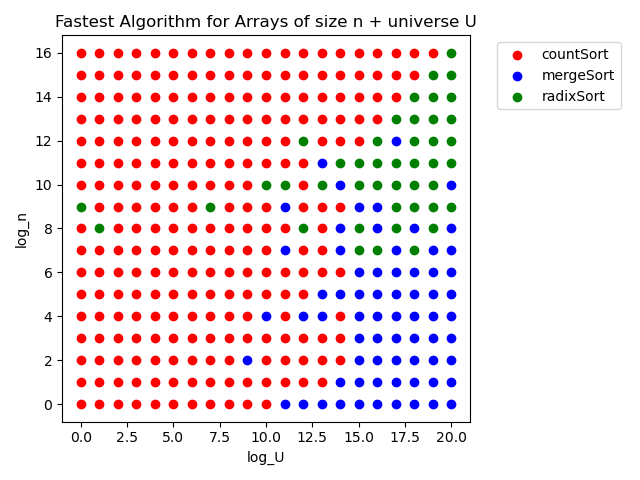
\includegraphics[]{fall2022/psets/ps1/algorithms_runtime_comparison.png} \\
            
            Above is the plot for the fastest sorting algorithm at various values of $n$ and $U$, representing the size of a randomly generated array and the maximum key value, respectively. Despite various possible implementation inefficiencies and a lack of optimization at every step for radixSort, the graph still displays a shape reflective of asymptotic theory. In particular, at low values of $U$ (and with large values of $n$), countSort displays the fastest runtime. Additionally, as the value of $U$ increases exponentially, mergeSort becomes the fastest algorithm, with radixSort being the fastest somewhere in between. While we may expect to see radixSort be the fastest at more times with an optimized implementation, regardless, the graph displays the general pattern we expect.
          
        \end{enumerate}

\end{enumerate}


\end{document}